\documentclass[border=4pt]{standalone}

\usepackage{tikz}

\definecolor{otblue}{HTML}{0072B2}
\definecolor{otorange}{HTML}{E69F00}
\definecolor{otteal}{HTML}{009E73}
\definecolor{otpurple}{HTML}{CC79A7}
\definecolor{otgray}{HTML}{5A5A5A}

\begin{document}
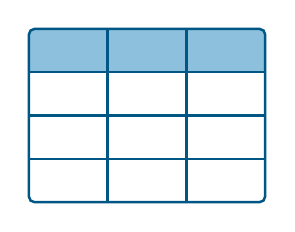
\begin{tikzpicture}[line width=0.9pt]
  \fill[otblue!45, rounded corners=2pt] (0,1.65) rectangle (3,2.2);
  \fill[otblue!45] (0,1.65) rectangle (3,1.9);
  \draw[draw=otblue!75!black, rounded corners=2pt] (0,0) rectangle (3,2.2);
  \foreach \y in {0.55,1.1,1.65}{\draw[otblue!75!black] (0,\y) -- (3,\y);}
  \foreach \x in {1,2}{\draw[otblue!75!black] (\x,0) -- (\x,2.2);}
\end{tikzpicture}
\end{document}
